

\documentclass[]{article}
%\usepackage[latin1]{inputenc}
\usepackage[utf8]{inputenc}
% Esto es para que el LaTeX sepa que el texto está en español:
%\usepackage[spanish]{babel}

% Paquetes de la AMS:
\usepackage{amsmath, amsthm, amsfonts}
\usepackage{graphicx}

%opening
\title{Trabajo Práctico 1}
\author{Jairo Jiménez \\
	Sergio De Raco}

\begin{document}

\maketitle


\section*{Objetivo}

\section*{Alcance}

\section*{Resultados esperados}

\section*{Metodología}

\section{Sobreajuste y poda}

El mejor ajuste del árbol se da cuando la confianza es de 0.1, después de este valor, empieza el sobreajuste del árbol, pues este deja baja la capacidad de pronosticar las nuevas instancias de manera correcta\\
A medida que aumenta la confianza, aumentan el tamaño y el número de hojas

%\begin{figure}
%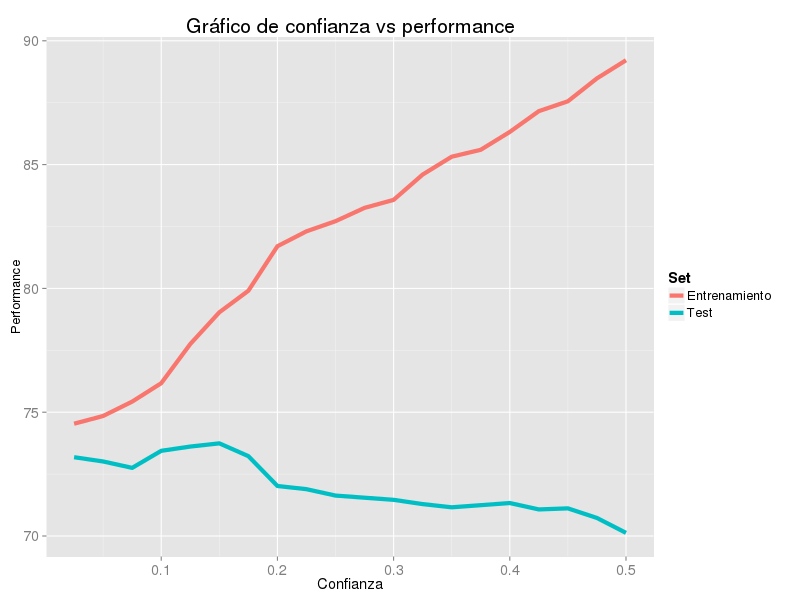
\includegraphics[width=0.8\linewidth,height=0.4\textheight]{Punto_1_Confianza_VS_ajuste}
%\caption[Confianza vs ajuste]{Confianza vs Ajuste}
%\label{P1ConfVSAjus}
%\end{figure}

\begin{figure}
	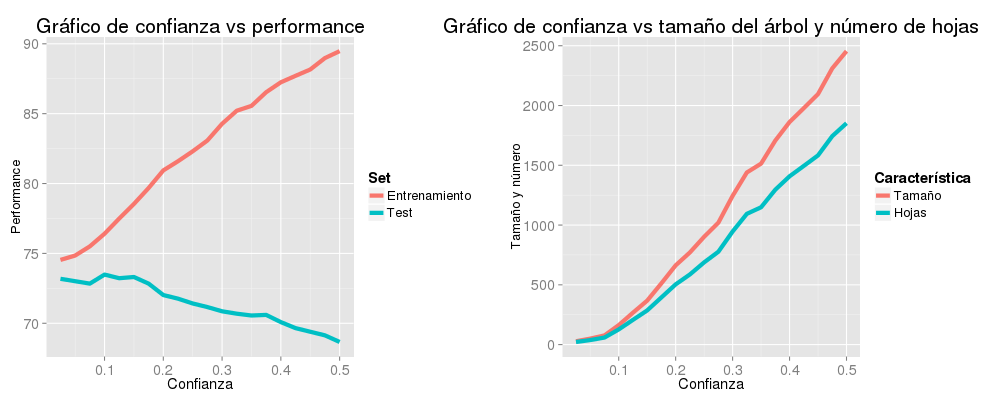
\includegraphics[scale = 0.4]{Punto_1_Graficos_Mezclados}
	\caption[Confianza vs ajuste]{Gráficos de confianza}
	\label{P1Conf}
\end{figure}


\begin{figure}
	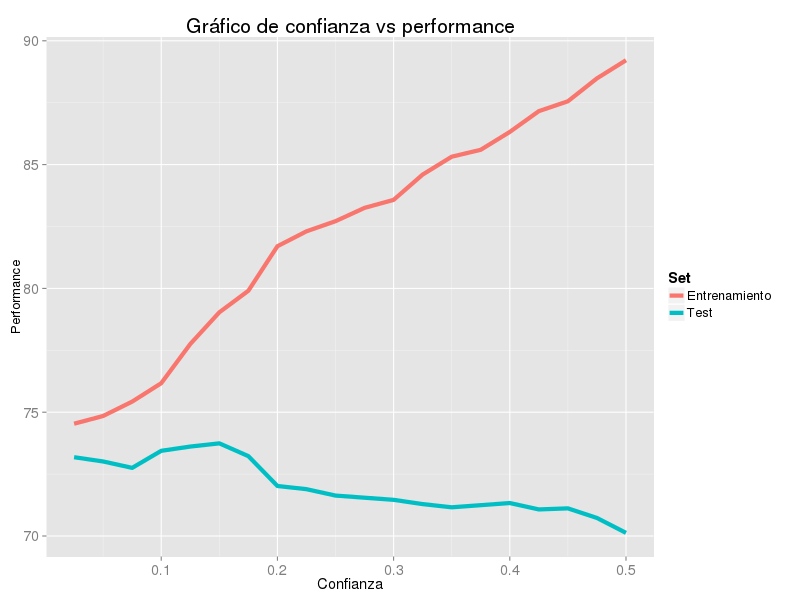
\includegraphics[scale = 0.4]{Punto_1_Confianza_VS_ajuste}
	\caption[Confianza vs ajuste]{Confianza vs Ajuste}
	\label{P1ConfVSAjus}
\end{figure}

\begin{figure}
	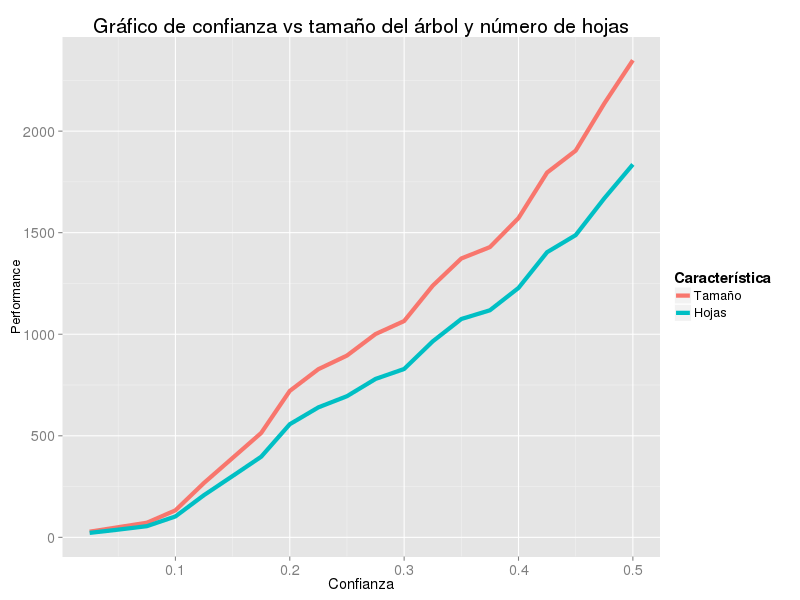
\includegraphics[scale = 0.4]{Punto_1_Confianza_VS_tamano}
	\caption[Confianza vs ajuste]{Confianza vs Tamaño}
	\label{P1ConfVSTamano}
\end{figure}





\section{Tratamiento de datos faltantes}

\section{Tolerancia al ruido}

\section{Discretización de atributos numéricos}

\section*{Conclusiones}

\section*{Trabajo futuro}

\bibliography{Bibliografia.bib}

\section*{Referencias}

\end{document}
